\documentclass[11pt,a4paper]{article}

\usepackage[margin=2.5cm]{geometry}
\usepackage{graphicx}
\usepackage{booktabs}
\usepackage{array}
\usepackage{tabularx}
\usepackage{amsmath}
\usepackage{hyperref}
\usepackage{listings}
\usepackage{caption}
\usepackage{subcaption}
\usepackage{xcolor}

\hypersetup{
    colorlinks=true,
    linkcolor=blue,
    urlcolor=blue,
    citecolor=blue
}

\lstset{
    basicstyle=\ttfamily\small,
    breaklines=true,
    frame=single,
    backgroundcolor=\color{gray!8}
}

\title{GPU Optimization of the\\``Isolated Ones'' Stencil Problem\\[0.4em]
\large From CUDA Exploration to HIP Implementation}
\author{Konstantin Kolchin}
\date{\today}

\begin{document}
\maketitle

\begin{abstract}
We study GPU kernels that count \emph{isolated} cells marked~$1$ in a binary
$N\times N$ matrix: a cell counts only if it equals~$1$ and all eight
neighbors (including diagonals) are~$0$, with the matrix border treated as~$0$.
Starting from a na\"ive per-thread implementation, we built a reproducible
benchmark harness in a Jupyter notebook (Numba CUDA on Google Colab, NVIDIA T4),
identified a tile-and-halo family of kernels (method~5) as the most promising
direction, and ported it to a standalone C++/HIP application for AMD ROCm.
The HIP port enabled LDS (shared-memory) micro-optimizations unavailable in the
Python notebook stack---including explicit bank padding, \texttt{uint32} row
packing, and warp shuffle---and was measured on an AMD Radeon RX~6800 XT
(\texttt{gfx1030}).
On NVIDIA, the na\"ive atomic baseline remains competitive for sparse inputs;
on AMD, the tiled LDS approach wins clearly ($\sim\!2.4\times$ at $N{=}1024$).
Simple variants outperformed ``textbook'' bitwise and shuffle extensions on
\texttt{gfx1030}, underscoring that optimizations must be validated per target
architecture.
Artifacts (notebook, HIP benchmark, plotting script) are at
\url{https://github.com/konkolchin/cuda-to-hip}.
\end{abstract}

\section{Problem statement}
\label{sec:problem}

The problem about isolated ones was stated during the interview by Tomasz.
Given a binary matrix $G$ of size $N\times N$ (stored as \texttt{uint8}), count
cells $(i,j)$ such that
\begin{equation}
  G_{i,j} = 1
  \quad\text{and}\quad
  \forall\,(di,dj) \in \{-1,0,1\}^2 \setminus \{(0,0)\}:\;
  G_{i+di,\,j+dj} = 0,
\end{equation}
where out-of-bounds neighbors are defined as~$0$.
This is \textbf{not} connected-component labeling: we count only cells that are
``$1$'' with an empty $3\times 3$ neighborhood (excluding the center).

A literal GPU translation assigns one thread per interior cell and increments a
global counter when the eight-neighbor test succeeds:
\begin{lstlisting}[language=C++]
if (mat[i][j] == 1
    && mat[i-1][j-1] == 0 && mat[i-1][j] == 0 && mat[i-1][j+1] == 0
    && mat[i][j-1] == 0                   && mat[i][j+1] == 0
    && mat[i+1][j-1] == 0 && mat[i+1][j] == 0 && mat[i+1][j+1] == 0)
    atomicAdd(&counter, 1);
\end{lstlisting}
This baseline is correct but inefficient on GPUs because of (i)~branch divergence
in the long \texttt{\&\&} chain, (ii)~global \texttt{atomicAdd} serialization on
hits, (iii)~repeated uncached global loads for neighbor reads, and (iv)~explicit
boundary guards on every neighbor test.

Our goal was to explore alternative kernel structures, measure them under
controlled sparsity regimes, and prepare a HIP implementation suitable for AMD
hardware.

\section{Phase I: CUDA exploration in Google Colab}
\label{sec:phase1}

\subsection{Experimental setup}

We implemented all kernels in Python using \textbf{Numba CUDA} inside a Jupyter
notebook (\texttt{isolated\_ones\_gpu\_colab.ipynb}) and executed benchmarks on
\textbf{Google Colab} with an \textbf{NVIDIA Tesla T4} (compute capability~7.5,
warp size~32).

\paragraph{Data layout.}
Matrices are always stored as dense \texttt{uint8} arrays of shape $N\times N$.
For kernels that need a zero border without per-thread boundary branches, we
also use a padded array of shape $(N{+}2)\times(N{+}2)$ with a one-cell zero halo.

\paragraph{Sparsity regimes.}
Each cell is independently set to~$1$ with probability equal to a \emph{density}
parameter. We benchmark three regimes:
\begin{itemize}
  \item \textbf{sparse} (density $=0.01$): few ones, many early exits;
  \item \textbf{medium} (density $=0.10$);
  \item \textbf{dense} (density $=0.90$): almost all cells are~$1$, few isolated.
\end{itemize}
Matrix sizes $N \in \{1024,\,2048\}$; each kernel timing uses warmup iterations
followed by repeated timed runs with device synchronization.

\paragraph{Correctness.}
Every GPU method is checked against a CPU reference implementation that
implements the same eight-neighbor rule.

\subsection{Method families explored}

We catalogued several design points (names preserved in the benchmark output):

\begin{table}[h]
  \centering
  \caption{Kernel families in the Colab notebook.}
  \label{tab:methods-colab}
  \begin{tabular}{@{}llp{7.2cm}@{}}
    \toprule
    ID & Name & Idea \\
    \midrule
    1  & \texttt{interview\_if\_atomic} & Literal \texttt{if (\&\&...)} + global atomic \\
    1b & \texttt{divergent\_early\_return} & Same logic, early \texttt{return} per check \\
    2  & \texttt{uniform\_block\_reduce} & Uniform neighbor-sum; per-block reduction \\
    3  & \texttt{compaction} & \texttt{flatnonzero} list of ones; sparse second pass \\
    4  & \texttt{warp\_ballot} & Uniform path; full block reduce (ballot N/A in Numba) \\
    5  & \texttt{tile30\_halo} & $30{\times}30$ tile, $32{\times}32$ halo in shared memory \\
    5b & \texttt{tile16\_halo} & $16{\times}16$ tile equals thread block (one thread/cell) \\
    5c & \texttt{tile30\_nbrcache} & Software cache: precompute 8-neighbor sum in LDS \\
    5d & \texttt{tile30\_block30} & $30{\times}30$ tile equals $30{\times}30$ block (900 threads) \\
    6  & \texttt{lut\_k3\_warp} & $k{=}3$ bitmask LUT in shared memory ($\sim$32\,MB table) \\
    \bottomrule
  \end{tabular}
\end{table}

\subsection{Why method~5 was selected}

Among the ``respectable fixes'' (methods~2--5), \textbf{method~5
(\texttt{tile30\_halo})} emerged as the most promising:
\begin{itemize}
  \item It loads a \textbf{halo tile once} into shared memory (CUDA shared / AMD
        LDS) and reuses it for up to $30\times 30 = 900$ interior cells per
        thread block.
  \item It avoids global atomics via a \textbf{block-local reduction}.
  \item It uses a \textbf{uniform neighbor-sum} test ($\sum$ neighbors $= 0$)
        instead of a deeply divergent \texttt{\&\&} tree.
  \item At $N{=}1024$ it launched $\lceil N/30\rceil^2 \approx 35^2 = 1225$
        blocks---\emph{fewer} than the $64^2 = 4096$ blocks of method~1---so it
        is not launch-bound in the same way as fine-grained bitmask/LUT schemes
        (method~6).
\end{itemize}

We applied a standard tiled-matrix lesson to reduce LDS bank conflicts:
row stride \texttt{SM\_STRIDE = HALO + 1 = 33} instead of~32 when indexing the
$32\times 32$ halo array.

\subsection{Colab (NVIDIA T4) results}

Figure~\ref{fig:colab} summarizes median kernel times from the notebook
benchmark on the T4.

\begin{figure}[htbp]
  \centering
  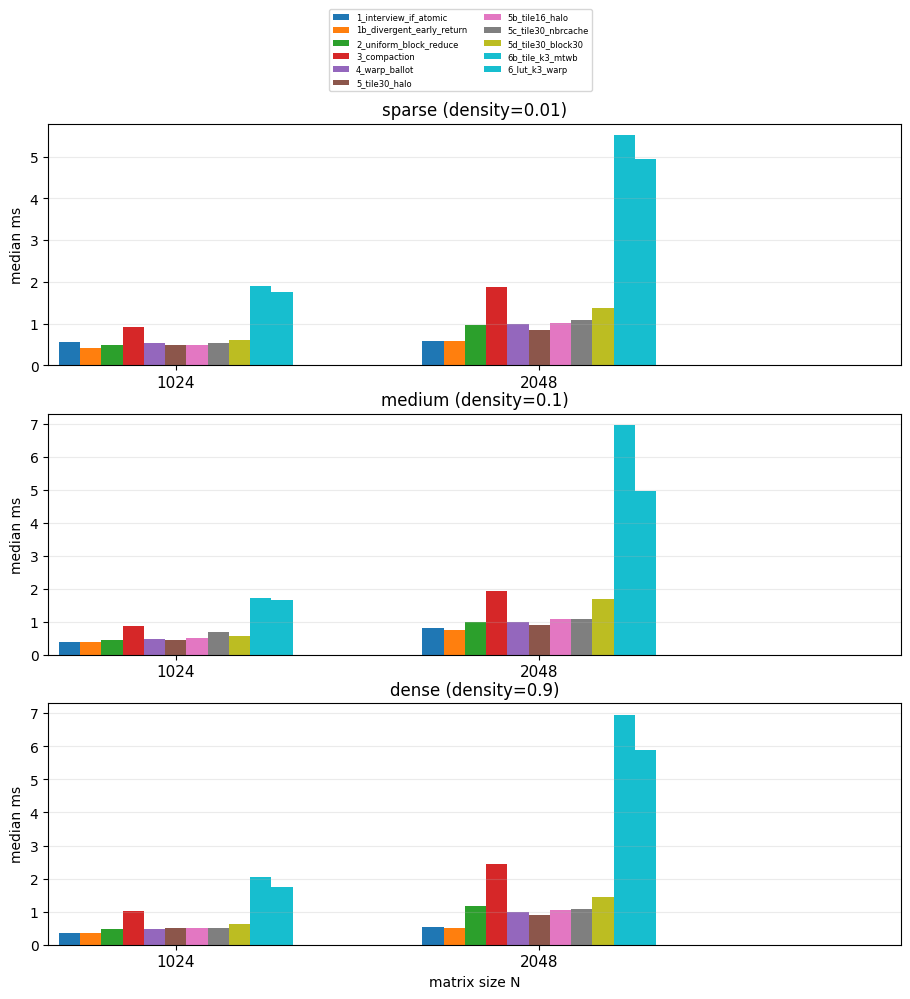
\includegraphics[width=\textwidth]{fig1.png}
  \caption{Median kernel time (ms) on \textbf{NVIDIA Tesla T4} (Google Colab),
           from the Jupyter/Numba CUDA notebook.
           One subplot per density regime; grouped bars for $N{=}1024$ and
           $N{=}2048$.}
  \label{fig:colab}
\end{figure}

\paragraph{Key observations on T4.}
For \textbf{sparse} inputs at $N{=}1024$, the na\"ive atomic kernels
(methods~1/1b) were often \textbf{fastest} or tied for first place: with only
$\sim$1\% ones, most threads exit immediately and few atomics fire.
Method~5 was typically within $\sim$10--20\% of method~1 ($\sim$0.46\,ms vs.\
$\sim$0.38--0.55\,ms)---respectable, but not the overall winner on NVIDIA for
sparse data.
Method~6 (LUT) was substantially slower due to very large block counts and table
pressure.
These results motivated a deeper implementation on native GPU C++ where
additional low-level features could be tested fairly.

\section{Phase II: C++/HIP testing application}
\label{sec:phase2}

\subsection{Motivation}

The notebook was excellent for rapid prototyping, but Numba CUDA imposes
limitations:
\begin{itemize}
  \item No \texttt{\_\_shfl\_sync} / warp shuffle intrinsics in the Python
        kernels we wrote.
  \item No convenient \texttt{uint32} bitwise halo packing in device code.
  \item Coarse timing via host \texttt{time.perf\_counter()} rather than
        \texttt{hipEvent} pairs on the device timeline.
  \item The CUDA \emph{simulator} mode (when Colab GPU quota is exhausted) does
        not faithfully model atomics or device memory for full validation.
\end{itemize}

We therefore built \texttt{hip\_isolated\_ones}: a standalone C++17/HIP
benchmark that reproduces the notebook's correctness checks and timing
methodology, targets \textbf{AMD ROCm} (tested on HIP~6.4), and adds kernel
variants that exploit features available in native GPU C++.

\subsection{Extensions in native C++/HIP (vs.\ the notebook)}

Table~\ref{tab:hip-ext} lists optimizations added in the HIP port but not
exercised in the Colab notebook.

\subsection{HIP-only features vs.\ CUDA portability}
\label{sec:hip-vs-cuda}

\textbf{Short answer: we did not rely on any API that exists only in HIP and is
absent from CUDA.}
HIP is deliberately a \emph{CUDA-compatible} portability layer: the kernels use
\texttt{\_\_shared\_\_}, \texttt{\_\_syncthreads()}, \texttt{atomicAdd},
\texttt{\_\_shfl}, and the triple-chevron launch syntax---all of which have
direct or near-direct CUDA counterparts (\texttt{cudaEvent} vs.\ \texttt{hipEvent},
\texttt{\_\_shfl\_sync} vs.\ \texttt{\_\_shfl})~\cite{hip-faq,hipify-device-api}.

What the C++/HIP application added over the notebook was therefore:
\begin{itemize}
  \item \textbf{Native device intrinsics} (\texttt{\_\_shfl} with explicit width)
        not exposed in our Numba CUDA Python kernels~\cite{hip-lang-ext};
  \item \textbf{Host runtime timing} via \texttt{hipEventRecord} /
        \texttt{hipEventElapsedTime} rather than host wall-clock
        timers~\cite{hip-events};
  \item \textbf{Full control} over thread-block geometry (e.g.\ a $(32,8)$ block
        for variant~\texttt{5g}) and \texttt{uint32} bit tricks in device code.
\end{itemize}

\paragraph{AMD-specific context (terminology and hardware).}
On AMD GPUs, on-chip shared memory is called \textbf{LDS} (Local Data
Share)~\cite{hip-prog-model}; our code still declares it with the portable
\texttt{\_\_shared\_\_} keyword.
HIP documents \emph{cross-lane} operations (shuffle, ballot) for wavefronts;
on many AMD parts the hardware wavefront is 64-wide, while our RX~6800 XT
reported \texttt{warpSize}${=}32$ in device properties---shuffle width
parameters (\texttt{width}${=}16$ or~$32$) remain meaningful~\cite{hip-lang-ext,hip-faq}.
These are portability and hardware-model considerations, not HIP-exclusive APIs
that CUDA lacks.
Further background is in the official {ROCm}/{HIP} documentation~\cite{hip-docs,rocm-prog-guide,hip-porting}.

\begin{table}[htbp]
  \centering
  \small
  \caption{Extensions in the HIP application beyond the notebook baseline.}
  \label{tab:hip-ext}
  \begin{tabularx}{\textwidth}{@{}>{\raggedright\arraybackslash}p{2.6cm}
                                   @{\hspace{1.2em}}
                                   >{\raggedright\arraybackslash}p{3.2cm}
                                   >{\raggedright\arraybackslash}X@{}}
    \toprule
    Variant & Mechanism & Rationale \\
    \midrule
    \texttt{5a\_tile30\_nopad} &
      Row stride $=32$ (no $+1$ pad) &
      A/B test for LDS bank conflicts \\
    \texttt{5e\_tile30\_u32pack} &
      Pack each 32-wide halo row into one \texttt{uint32} &
      Fewer, wider LDS accesses; bit tests for neighbors \\
    \texttt{5g\_tile30\_u32pack\_shfl} &
      \texttt{uint32} rows + \texttt{\_\_shfl} for left/right &
      Pass horizontal neighbors between lanes \\
    \texttt{5f\_tile16\_shfl} &
      Tile-$=$block $16{\times}16$ + 16-wide shuffle groups &
      Clean mapping of row threads to shuffle width \\
    (all) &
      \texttt{hipEvent} timing, 5 warmup runs &
      Stable GPU-side timing \\
    \bottomrule
  \end{tabularx}
\end{table}

\subsection{Benchmark protocol on AMD}

Hardware: \textbf{AMD Radeon RX~6800 XT}, architecture \texttt{gfx1030}, ROCm
6.4, \texttt{hipcc} (AMD clang~19).
Reported \texttt{warpSize} from the runtime: \textbf{32} (relevant for shuffle
width).
Same matrix sizes, densities, and seeded random grids as Phase~I.
Each method: \textbf{5 untimed warmup} launches, then \textbf{20 timed}
iterations; we record \textbf{median and mean} milliseconds (\texttt{hipEvent}
elapsed time, including synchronization).

\section{Results on AMD RX 6800 XT}
\label{sec:results-amd}

Tables~\ref{tab:amd-1024-sparse}--\ref{tab:amd-2048-dense} list the median kernel
times (ms) for all six benchmark scenarios on the RX~6800 XT: matrix sizes
$N \in \{1024,\,2048\}$ crossed with densities sparse ($0.01$), medium ($0.10$),
and dense ($0.90$).
The same six scenarios are visualized in Figure~\ref{fig:hip}; the bar chart
omits \texttt{5e} and \texttt{5g} for readability (those rows appear in the
tables).

\begin{figure}[htbp]
  \centering
  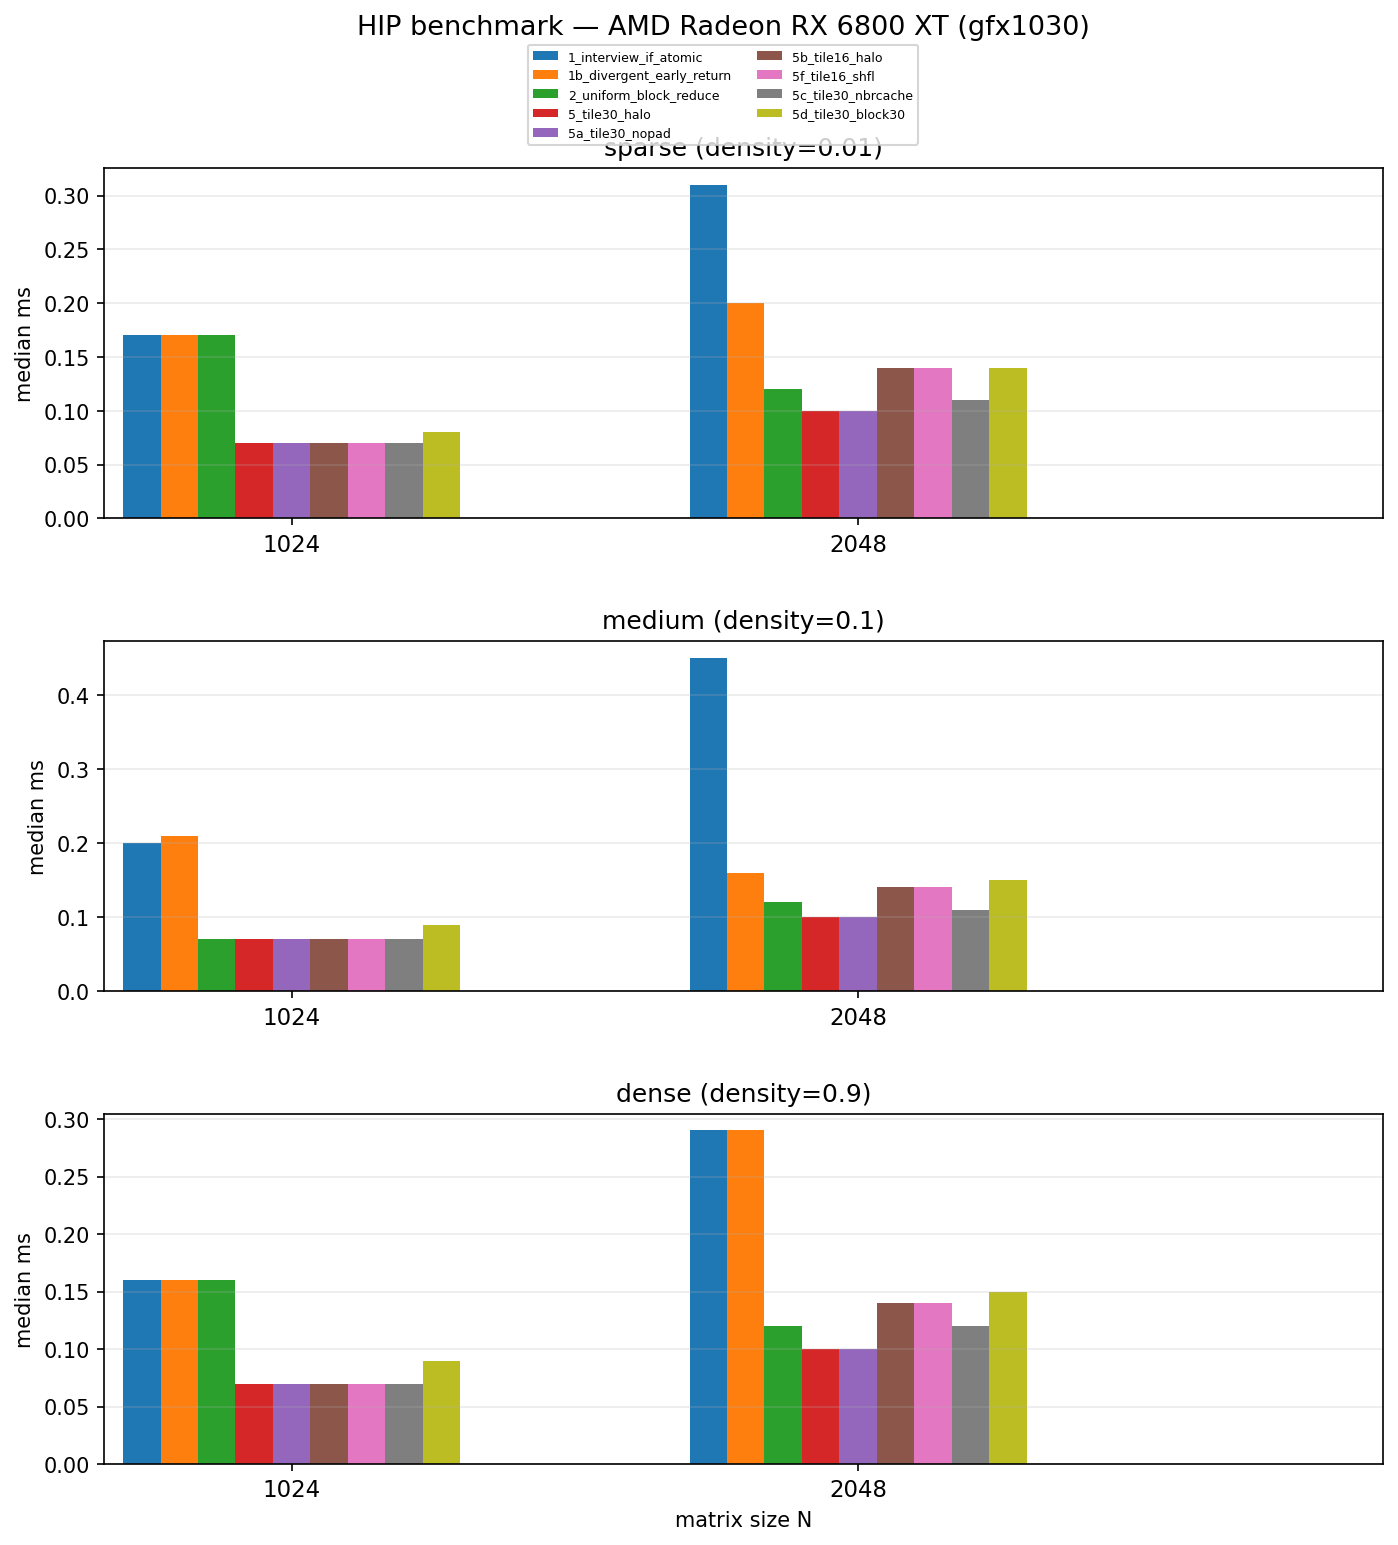
\includegraphics[width=\textwidth]{fig2.png}
  \caption{Median kernel time (ms) on \textbf{AMD Radeon RX~6800 XT}
           (\texttt{gfx1030}), from the C++/HIP application
           (\texttt{hip\_isolated\_ones}).
           One subplot per density regime; grouped bars for $N{=}1024$ and
           $N{=}2048$, corresponding to
           Tables~\ref{tab:amd-1024-sparse}--\ref{tab:amd-2048-dense}.
           Variants \texttt{5e} and \texttt{5g} excluded from the plot (slower).}
  \label{fig:hip}
\end{figure}

\subsection{Detailed median timings (six scenarios)}

% --- N = 1024 ---
\begin{table}[htbp]
  \centering
  \footnotesize
  \caption{RX~6800 XT: $N=1024$, sparse (density $=0.01$). Median kernel time (ms).}
  \label{tab:amd-1024-sparse}
  \begin{tabular}{@{}p{5.1cm}r@{}}
    \toprule
    Method & median (ms) \\
    \midrule
    \texttt{1\_interview\_if\_atomic}      & 0.17 \\
    \texttt{1b\_divergent\_early\_return} & 0.17 \\
    \texttt{2\_uniform\_block\_reduce}    & 0.17 \\
    \texttt{5\_tile30\_halo}              & 0.07 \\
    \texttt{5a\_tile30\_nopad}            & 0.07 \\
    \texttt{5e\_tile30\_u32pack}          & 0.12 \\
    \texttt{5g\_tile30\_u32pack\_shfl}    & 0.10 \\
    \texttt{5b\_tile16\_halo}              & 0.07 \\
    \texttt{5f\_tile16\_shfl}             & 0.07 \\
    \texttt{5c\_tile30\_nbrcache}          & 0.07 \\
    \texttt{5d\_tile30\_block30}          & 0.08 \\
    \bottomrule
  \end{tabular}
\end{table}

\begin{table}[htbp]
  \centering
  \footnotesize
  \caption{RX~6800 XT: $N=1024$, medium (density $=0.10$). Median kernel time (ms).}
  \label{tab:amd-1024-medium}
  \begin{tabular}{@{}p{5.1cm}r@{}}
    \toprule
    Method & median (ms) \\
    \midrule
    \texttt{1\_interview\_if\_atomic}      & 0.20 \\
    \texttt{1b\_divergent\_early\_return} & 0.21 \\
    \texttt{2\_uniform\_block\_reduce}    & 0.07 \\
    \texttt{5\_tile30\_halo}              & 0.07 \\
    \texttt{5a\_tile30\_nopad}            & 0.07 \\
    \texttt{5e\_tile30\_u32pack}          & 0.11 \\
    \texttt{5g\_tile30\_u32pack\_shfl}    & 0.10 \\
    \texttt{5b\_tile16\_halo}              & 0.07 \\
    \texttt{5f\_tile16\_shfl}             & 0.07 \\
    \texttt{5c\_tile30\_nbrcache}          & 0.07 \\
    \texttt{5d\_tile30\_block30}          & 0.09 \\
    \bottomrule
  \end{tabular}
\end{table}

\begin{table}[htbp]
  \centering
  \footnotesize
  \caption{RX~6800 XT: $N=1024$, dense (density $=0.90$). Median kernel time (ms).}
  \label{tab:amd-1024-dense}
  \begin{tabular}{@{}p{5.1cm}r@{}}
    \toprule
    Method & median (ms) \\
    \midrule
    \texttt{1\_interview\_if\_atomic}      & 0.16 \\
    \texttt{1b\_divergent\_early\_return} & 0.16 \\
    \texttt{2\_uniform\_block\_reduce}    & 0.16 \\
    \texttt{5\_tile30\_halo}              & 0.07 \\
    \texttt{5a\_tile30\_nopad}            & 0.07 \\
    \texttt{5e\_tile30\_u32pack}          & 0.12 \\
    \texttt{5g\_tile30\_u32pack\_shfl}    & 0.10 \\
    \texttt{5b\_tile16\_halo}              & 0.07 \\
    \texttt{5f\_tile16\_shfl}             & 0.07 \\
    \texttt{5c\_tile30\_nbrcache}          & 0.07 \\
    \texttt{5d\_tile30\_block30}          & 0.09 \\
    \bottomrule
  \end{tabular}
\end{table}

% --- N = 2048 ---
\begin{table}[htbp]
  \centering
  \footnotesize
  \caption{RX~6800 XT: $N=2048$, sparse (density $=0.01$). Median kernel time (ms).}
  \label{tab:amd-2048-sparse}
  \begin{tabular}{@{}p{5.1cm}r@{}}
    \toprule
    Method & median (ms) \\
    \midrule
    \texttt{1\_interview\_if\_atomic}      & 0.31 \\
    \texttt{1b\_divergent\_early\_return} & 0.20 \\
    \texttt{2\_uniform\_block\_reduce}    & 0.12 \\
    \texttt{5\_tile30\_halo}              & 0.10 \\
    \texttt{5a\_tile30\_nopad}            & 0.10 \\
    \texttt{5e\_tile30\_u32pack}          & 0.22 \\
    \texttt{5g\_tile30\_u32pack\_shfl}    & 0.21 \\
    \texttt{5b\_tile16\_halo}              & 0.14 \\
    \texttt{5f\_tile16\_shfl}             & 0.14 \\
    \texttt{5c\_tile30\_nbrcache}          & 0.11 \\
    \texttt{5d\_tile30\_block30}          & 0.14 \\
    \bottomrule
  \end{tabular}
\end{table}

\begin{table}[htbp]
  \centering
  \footnotesize
  \caption{RX~6800 XT: $N=2048$, medium (density $=0.10$). Median kernel time (ms).}
  \label{tab:amd-2048-medium}
  \begin{tabular}{@{}p{5.1cm}r@{}}
    \toprule
    Method & median (ms) \\
    \midrule
    \texttt{1\_interview\_if\_atomic}      & 0.45 \\
    \texttt{1b\_divergent\_early\_return} & 0.16 \\
    \texttt{2\_uniform\_block\_reduce}    & 0.12 \\
    \texttt{5\_tile30\_halo}              & 0.10 \\
    \texttt{5a\_tile30\_nopad}            & 0.10 \\
    \texttt{5e\_tile30\_u32pack}          & 0.23 \\
    \texttt{5g\_tile30\_u32pack\_shfl}    & 0.21 \\
    \texttt{5b\_tile16\_halo}              & 0.14 \\
    \texttt{5f\_tile16\_shfl}             & 0.14 \\
    \texttt{5c\_tile30\_nbrcache}          & 0.11 \\
    \texttt{5d\_tile30\_block30}          & 0.15 \\
    \bottomrule
  \end{tabular}
\end{table}

\begin{table}[htbp]
  \centering
  \footnotesize
  \caption{RX~6800 XT: $N=2048$, dense (density $=0.90$). Median kernel time (ms).}
  \label{tab:amd-2048-dense}
  \begin{tabular}{@{}p{5.1cm}r@{}}
    \toprule
    Method & median (ms) \\
    \midrule
    \texttt{1\_interview\_if\_atomic}      & 0.29 \\
    \texttt{1b\_divergent\_early\_return} & 0.29 \\
    \texttt{2\_uniform\_block\_reduce}    & 0.12 \\
    \texttt{5\_tile30\_halo}              & 0.10 \\
    \texttt{5a\_tile30\_nopad}            & 0.10 \\
    \texttt{5e\_tile30\_u32pack}          & 0.23 \\
    \texttt{5g\_tile30\_u32pack\_shfl}    & 0.22 \\
    \texttt{5b\_tile16\_halo}              & 0.14 \\
    \texttt{5f\_tile16\_shfl}             & 0.14 \\
    \texttt{5c\_tile30\_nbrcache}          & 0.12 \\
    \texttt{5d\_tile30\_block30}          & 0.15 \\
    \bottomrule
  \end{tabular}
\end{table}

\subsection{Cross-platform comparison}

\begin{table}[h]
  \centering
  \caption{Qualitative ranking shift: sparse, $N{=}1024$.}
  \label{tab:cross}
  \begin{tabular}{@{}lll@{}}
    \toprule
    Platform & Winner (sparse) & Method~5 vs.\ baseline \\
    \midrule
    NVIDIA T4 (Colab)  & Methods~1/1b $\approx$ best & $\sim$0.46\,ms vs.\ $\sim$0.4\,ms (5 slightly slower) \\
    AMD RX~6800 XT     & \textbf{Method~5 family}    & $\sim$0.07\,ms vs.\ $\sim$0.17\,ms (\textbf{$\sim$2.4$\times$ faster}) \\
    \bottomrule
  \end{tabular}
\end{table}

\section{Discussion}
\label{sec:discussion}

\paragraph{Method~5 wins on AMD.}
The tile-and-halo pattern amortizes one LDS load over hundreds of cells and
replaces global atomics with block reductions.
On \texttt{gfx1030} this dominates the na\"ive approach for \emph{all} density
regimes at $N{=}1024$, including sparse data where NVIDIA favored early-exit
atomics.

\paragraph{Bank padding (\texttt{5} vs.\ \texttt{5a}).}
\texttt{SM\_STRIDE = HALO + 1} is the standard remedy for 32-way shared-memory
bank conflicts when warps walk along rows.
On RX~6800 XT, \texttt{5} and \texttt{5a} were \textbf{identical} within
measurement resolution---the padding lesson is still worth stating in design
reviews even when a particular kernel is not conflict-limited.

\paragraph{Bitwise pack and shuffle (\texttt{5e}, \texttt{5g}, \texttt{5f}).}
These extensions are natural ``next steps'' when moving from Python to HIP.
On \texttt{gfx1030}, \texttt{5e}/\texttt{5g} were \textbf{slower} than plain
\texttt{5}: the cost of building \texttt{uint32} row words and the altered
thread-block geometry outweighed saved LDS traffic.
\texttt{5f} matched \texttt{5b}---shuffle did not help for the $16{\times}16$
tile-equals-block layout at these problem sizes.

\paragraph{Neighbor-sum cache (\texttt{5c}).}
Precomputing the eight-neighbor sum for every cell helps when many cells are~$1$
(dense), but always pays for empty cells.
It tied with \texttt{5} at $N{=}1024$ and was marginally slower at $N{=}2048$.

\paragraph{Large thread blocks (\texttt{5d}).}
Using a $30{\times}30 = 900$-thread block removes the stride loop but increased
sync pressure and slightly hurt performance vs.\ the 256-thread \texttt{5}
kernel.

\paragraph{Method~1b anomaly at $N{=}2048$ medium.}
Early-return layout (\texttt{1b}) reported a much lower median than the single
\texttt{if} form (\texttt{1}) in one full sweep ($\sim$0.16\,ms vs.\ $\sim$0.45\,ms),
while other regimes showed parity.
With additional warmup and reporting both mean and median, \texttt{1b} remained
fast in that scenario; high variance in some repeated runs suggests sensitivity
to GPU clock behavior for the atomic path under medium density.
We treat \textbf{method~5} as the stable, architecture-agnostic headline result.

\section{Conclusions}
\label{sec:conclusions}

\begin{enumerate}
  \item The isolated-ones stencil is a compact but rich GPU micro-benchmark:
        it exposes divergence, atomics, LDS tiling, occupancy, and
        cross-vendor ranking reversals.
  \item Systematic exploration in a Colab Jupyter notebook identified
        \textbf{method~5 (tile30 halo + LDS + block reduce)} as the most
        promising structure, competitive on NVIDIA T4 but not always fastest on
        sparse inputs.
  \item A native \textbf{C++/HIP} port on AMD RX~6800 XT validated that method~5
        is \textbf{dominant on \texttt{gfx1030}} ($\sim$2.4$\times$ over the
        atomic baseline at $N{=}1024$ sparse).
  \item Native C++ device features (\texttt{uint32} packing, \texttt{\_\_shfl})
        must be profiled per GPU: on this hardware, simpler LDS tiling won.
        These intrinsics are available in CUDA as well; the gain was over the
        Python notebook, not over CUDA as a language.
  \item Artifacts: Jupyter notebook
        (\texttt{isolated\_ones\_gpu\_colab.ipynb}), HIP benchmark
        (\texttt{hip\_isolated\_ones/}), and plotting script
        (\texttt{plot\_benchmark.py}) are version-controlled for reproducibility.
\end{enumerate}

\section*{Artifacts and reproduction}

\begin{itemize}
  \item \textbf{Notebook:} \texttt{isolated\_ones\_gpu\_colab.ipynb} --- Numba
        CUDA kernels, CPU reference, Colab benchmark.
  \item \textbf{HIP app:} \texttt{hip\_isolated\_ones/} --- build with
        \texttt{make ARCH=gfx1030}, run \texttt{./hip\_isolated\_ones}.
  \item \textbf{Plot:} \texttt{python plot\_benchmark.py --input benchmark.txt}
        parses stdout and reproduces bar charts.
  \item \textbf{Repository:} \url{https://github.com/konkolchin/cuda-to-hip}
\end{itemize}

\bibliographystyle{plainurl}
\bibliography{references}

\end{document}
